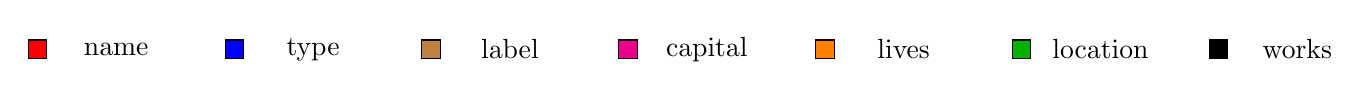
\begin{tikzpicture}
    \node[draw,fill=red] (nameColor) {};
    \node[right of = nameColor] (name) {name};

    \node[draw,fill=blue,right of = name,xshift=.5cm] (typeColor) {};
    \node[right of = typeColor] (type) {type};

    \node[draw,fill=brown,right of = type,xshift=.5cm] (labelColor) {};
    \node[right of = labelColor] (label) {label};

    \node[draw,fill=magenta,right of = label,xshift=.5cm] (capitalColor) {};
    \node[right of = capitalColor] (capital) {capital};

    \node[draw,fill=orange,right of = capital,xshift=.5cm] (livesColor) {};
    \node[right of = livesColor] (lives) {lives};

    \node[draw,fill=black!30!green,right of = lives,xshift=.5cm] (locationColor) {};
    \node[right of = locationColor] (location) {location};

    \node[draw,fill=black,right of = location,xshift=.5cm] (worksColor) {};
    \node[right of = worksColor] (works) {works};
\end{tikzpicture}
%% vim: et:sw=4
